\chapter{Reconfigurable Network Analytics}
\label{cap:rna}

In this chapter, we present an extended version of the Reconfigurable Network Analytics (RNA), an approach for offloading some of Zeek's operations discussed in Section \ref{sec:bg:zeek_candidate_operations} to programmable forwarding devices compatible with P4. This proposal is an extended version of the Reconfigurable Network Analytics (RNA) framework, which was initially proposed by Ilha \cite{Ilha2022}. Since we advance on the original RNA, we describe the solution resulting from both, highlighting the new functionality.

\begin{figure}[h]
    \caption{RNA Framework}
    \begin{center}
        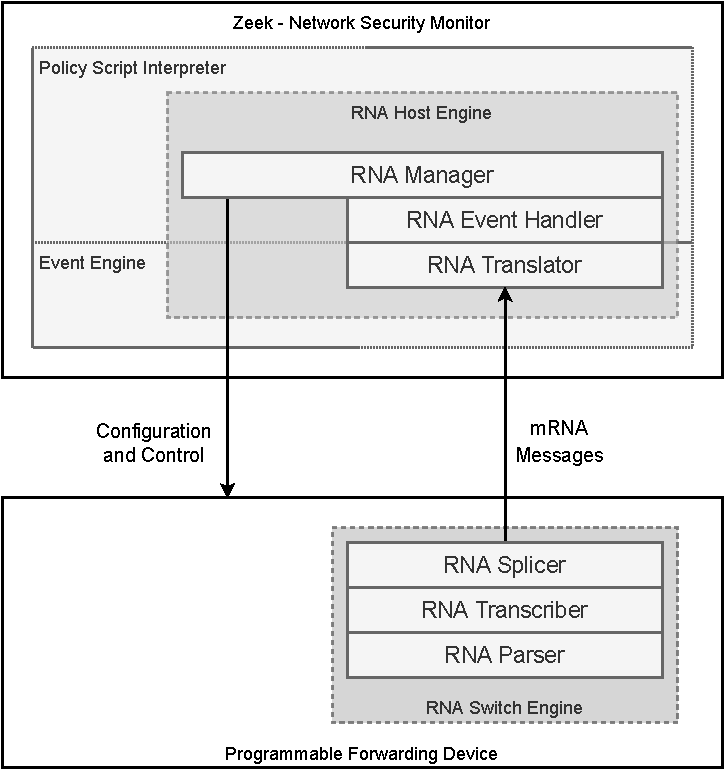
\includegraphics[width=0.7\textwidth]{images/arch_high_level.pdf}  
    \end{center}
    \label{fig:arch_high_level}
    \legend{Source: adapted from Ilha \cite{Ilha2022}}
\end{figure}

Figure \ref{fig:arch_high_level} illustrates the RNA framework. It is composed of two high-level components: the RNA Host Engine, which executes in one of Zeek's work nodes inside the IDS; and the RNA Switch Engine, which is executed in a P4 switch. Both components work together to offload packet analysis from Zeek to a programmable forwarding device. The RNA Switch Engine is able to parse packets and identify some of their characteristics, which are then summarized and sent to the RNA Host Engine. This summarized message is called mRNA. When the IDS receives this message, it is first processed by our Host Engine. It then converts the summarized message into Zeek's native structures, which can then be forwarded to Zeek's normal processing pipeline. This procedure allows us to bypass some operations that would be costly (such as protocol parsing and state tracking), and deliver this information closer or even directly to the Policy Script Interpreter (PSI, Section \ref{sec:bg:zeek_psi}), without disturbing Zeek's flow. By doing so, we make it that no change is required on existing scripts running on the PSI.

% TODO: check what to call this "'custom software' to be executed both...."
In the original concept of RNA, depending on the IDS scripts chosen to be monitored by the operator, it is necessary to develop custom software to be executed both by the Host Engine and the Switch Engine. This ad-hoc development process quickly becomes impractical when we increase the number of desired scripts to be offloaded. For this reason, we propose an automatic code generation mechanism, described later in Chapter \ref{cap:code_gen}, which allows RNA to be a modular solution, where varying combinations of Zeek scripts can be chosen to be monitored, without the need to develop new software. Before detailing this automated process, we briefly review the operation of RNA components.

% ==============================================================================
%                               RNA OVERVIEW
% ==============================================================================
\section{RNA Components in a Nutshell}
\label{sec:rna:overview}

Using Figure \ref{fig:arch_high_level} as reference, we present the high-level components of the RNA framework and their functionality. We start with the RNA Host Engine, since it is the controlling part of the whole deployment, and then we describe the RNA Switch Engine.

% TODO: check if we'll remove the "RNA Event Handler" completely, or say it was removed but exists in the original RNA
The Host Engine unfolds into three components. The RNA Manager is the controlling component of the deployment, which first configures the P4 switch, setting up a monitoring session and loading all P4 code that is required to execute the offloaded tasks. After configuring the switch, it registers all RNA Translators (one per-protocol of interest), so they receive mRNA messages. Translators are components responsible for waiting for such mRNA messages and translating them to Zeek native structures, and using those structures to trigger events, which are then consumed by the running scripts. The RNA Event Handler is another component that runs on the PSI and is initialized by the RNA Manager. It is designed as a debugging and logging component, capturing and handling events generated by the Translators.

The RNA Switch Engine is the program that executes in our P4-compatible programmable forwarding device. It has two components and we'll be following the route of an incoming packet to explain them. The first component that processes a packet is the RNA Parser. It parses and extracts headers from each protocol, from the link layer, up to the application layer if required. After all the headers have been extracted, the packet enters P4's ingress pipeline, where the RNA Transcriber is executed. It extracts useful information from the packet and sets metadata that later will be used to build our summarized message, while also filtering some undesired packets. Having all the required metadata and going into P4's egress pipeline, the RNA Splicer builds and sends our summarized message, the mRNA, to the Host Engine with all information it may require to trigger a native Zeek Event.

Another important structure is the mRNA Message. It is a summary of a packet, summarizing all the information that the Switch Engine was able to extract from it. Sending an mRNA message is more efficient than sending a whole packet because the original packet contains headers that would still need to be parsed, information that, in come cases, is not necessary, and is not validated. In the summarized message, all information from L2 up to the L7 layer is gathered, filtered, and, in some cases, even formatted according to Zeek's native structures, saving Zeek from doing these operations on its own. The information-gathering process still needs to happen, but it does in the Switch Engine, which runs in a purpose-built device, making it much more efficient for this task. So the more information the switch is able to extract, the less Zeek has to do.

In an ideal world scenario, we would like to extract all information that Zeek needs to trigger an event, but sometimes that is not possible. Zeek's internal structures track connection states and use detection heuristics, which, because of P4's limited processing power for general tasks, we are unable to implement. This requires the mRNA message to be modular, allowing us to send, together with it, a part of the packet that was not able to be processed in the switch. This ensures P4 extracts all information it can, leaving the rest for Zeek to finish analyzing.

% ==============================================================================
%                               RNA DETAILED ARCHITECTURE
% 
%  This includes modifications made to allow code generation
% ==============================================================================
% TODO: Change the name of this section
\section{Detailed Framework Design}
\label{sec:rna:detailed_design}

This proposed version of the RNA framework, different from the original framework, goes further and specifies another level of modules that make the framework adaptable to variable situations with varying sets of monitoring scripts. Before explaining the inner details of the framework, we will introduce two concepts that are fundamental for its understanding and will serve later as inputs for our code generator tool. Those concepts are \ProtocolTemplate{} and \Offloader{}:

\begin{itemize}
    \item An \textit{\Offloader{}} is a set of files and settings that allows RNA to offload a new script. Like the idea of a module, it can be added and removed to the deployment, without needing to develop new software or change existing components.

    \item A \textit{\ProtocolTemplate{}} is a set of files and settings that allows RNA to parse a new protocol. An \Offloader{} requires a set of \ProtocolTemplates{} to be able to parse and offload the desired scripts.
\end{itemize}

\begin{figure}[H]
    \caption{RNA Framework - Detailed view}
    \begin{center}
        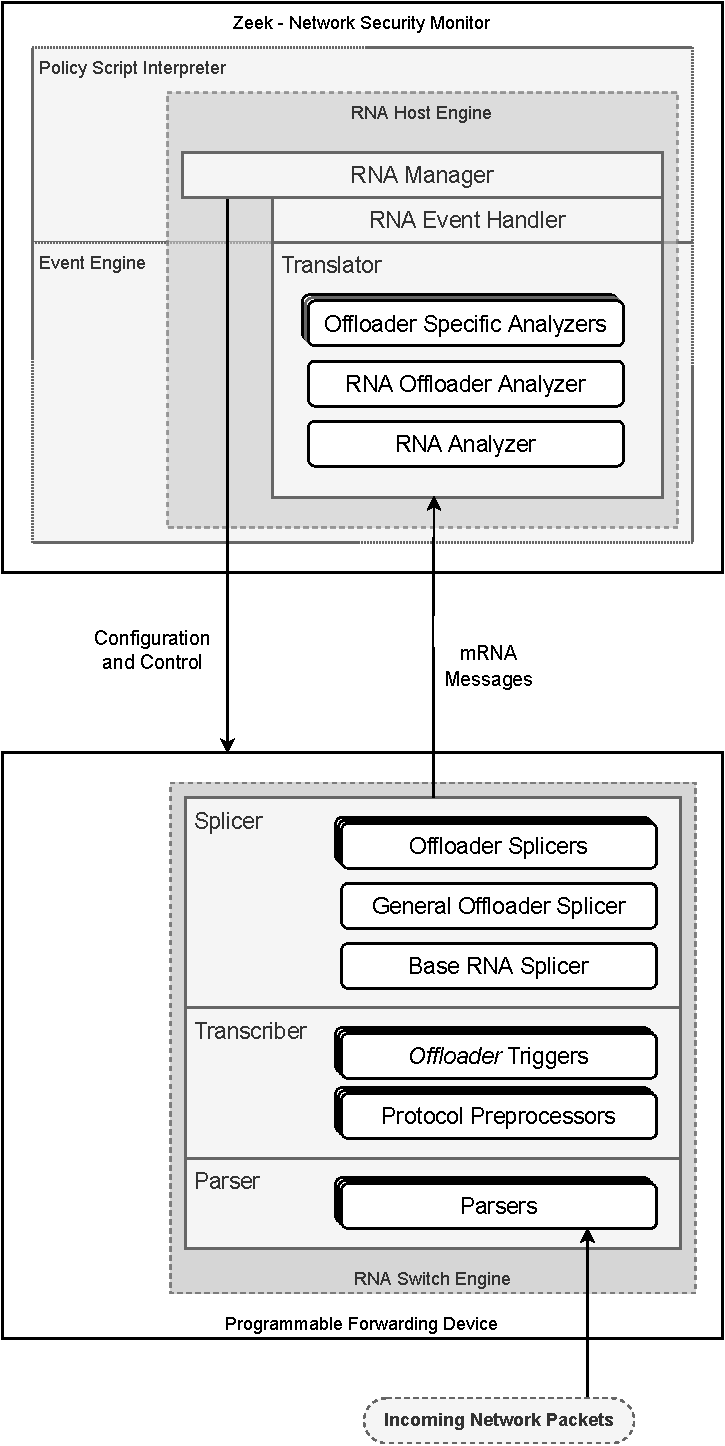
\includegraphics[width=0.6\textwidth]{images/arch_low_level.pdf}  
    \end{center}
    \label{fig:arch_low_level}
    \legend{Source: the author}
\end{figure}

In order to explain the details of the architecture behind the RNA, presented in Figure \ref{fig:arch_low_level}, we use an example of an incoming ICMPv4 ping (\textsc{ICMP Echo Request}) packet and its trajectory through a deployed instance of RNA. In this fictional deployed system, the network operator also offloads other scripts that monitor protocols such as ARP, TCP, and UDP, which are not triggered by this specific incoming ping packet.

\subsection{Switch Engine}

% Do we need this? Subsubsection directly after subsection.
\subsubsection*{The RNA Parser}

As the packet arrives at the P4-switch, it is first processed by the programmable parser. The RNA Parser component is a state machine with all the parsers the \Offloaders{} may need. Each one extracts its headers from the packet, and forwards the payload to the next parser. Each protocol's states and parsing instructions are provided by the \ProtocolTemplate{} of that specific protocol.

In our example which is shown in Figure \ref{fig:icmp_ex_parser}, the first parser would be the Ethernet parser, extracting its header, followed by the IPv4 and ICMP parsers. In the same figure, we also display other states of parsers that were not triggered, such as ARP, TCP, and UDP, each one provided by its own template. These unused protocol parsers are displayed by dotted lines, exemplifying where they would be linked in the general parser. After the packet's headers are parsed, it is sent to the ingress pipeline, where the RNA Transcriber will process the incoming data.

\begin{figure}[ht]
    \caption{Parsing States - ICMP Parsing Example}
    \begin{center}
        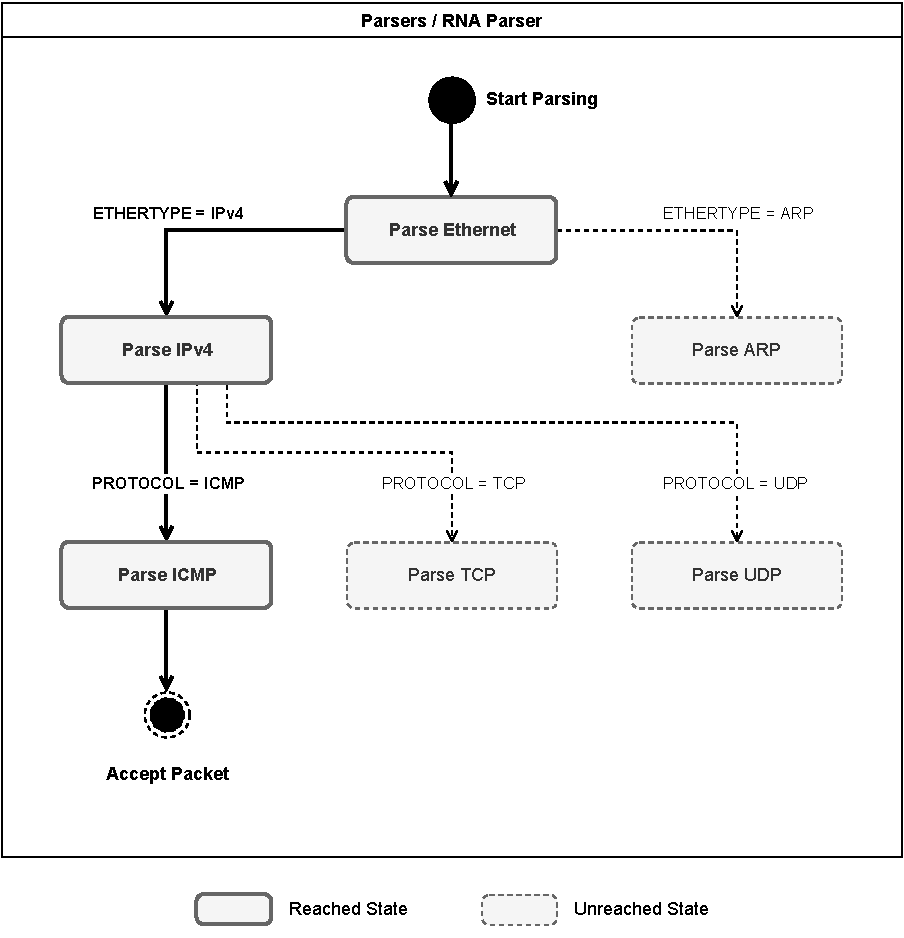
\includegraphics[width=0.7\textwidth]{images/icmp_ex_parser.pdf}  
    \end{center}
    \label{fig:icmp_ex_parser}
    \legend{Source: the author}
\end{figure}

\subsubsection*{RNA Transcriber}

In the RNA Transcriber, as shown in Figure \ref{fig:arch_low_level}, there are two types of modules, the Protocol Preprocessors, and the Offloader Triggers, both of which may have multiple instances. We start explaining the Protocol Preprocessors since they are the first modules to be executed inside this component.

The Protocol Preprocessors are functions that every \ProtocolTemplate{} may execute to extract protocol-related information from the packet, and save it to the metadata. This module is optional and every \ProtocolTemplate{} may have only one preprocessor. In our example, the processor extracts the ICMP type from the header and saves it in the metadata.

The next modules to be executed in the Transcriber are the Offloader Triggers, which are conditions that identify which \Offloader{} should be triggered. Each of these conditions is checked, and the first \Offloader{} to have its trigger condition valid is marked as the triggered one in the packet's metadata. In our example of an ICMP echo request, our trigger condition is \texttt{icmp.type = 8}. This ensures the \Offloader{} \textsc{ICMP Echo Request} is triggered when a ping packet has arrived.

% TODO: Maybe add here a code snippet

After a valid \Offloader{} is found, a copy of this packet is created, and using this cloned packet, the switch will be able to construct the mRNA message. The original packet will follow its flow and be delivered to the originally intended destination.

\subsubsection*{RNA Splicer}

The RNA Splicer is executed after the packet leaves the ingress pipeline and it enters the egress pipeline\footnotemark{}. The RNA Splicer is composed of three different types of Splicers, the RNA Base Splicer, the General Offloader Splicer, and the Offloader Splicers.

The RNA Base Splicer constructs the base header for the mRNA message. This is a simple header that contains the RNA version and the RNA message type. We decided to use this simple header to allow for more expandability in the future, for example, adding debugging and other types of messages.

% TODO: add code snippet of the header?

The next splicer, The General Offloader Splicer, constructs a header that contains general information, which all \Offloaders{} share, and is executed for every \Offloader{}. This information includes, for example, source IP, destination IP, L3, and L4 protocols, and triggered \Offloader{}. In our example of the ICMP ping request, the General Offloader Splicer sets both source and destination IPs, the L3 protocol to \texttt{IPv4}, the L4 protocol to \texttt{ICMP}, and the offloader type to \textsc{ICMP Echo Request}.

The third type of splicer is the Offloader Splicers. These are splicers that every \Offloader{} has. Each \Offloader{} Splicer constructs the header with the extra information required to execute its functionality, that was not yet present in the General Offloader Splicer. In our example, the \textsc{ICMP Echo Request} Splicer will construct a header with information about the ICMP ping packet: \texttt{type}, \texttt{code}, \texttt{sequence}, and \texttt{id}.

% TODO: Maybe add code snippets here too


\footnotetext{Since we are explaining the architecture behind RNA, we are not considering the inner workings of the programmable data plane, where a buffer connects the ingress and egress pipeline.}

After every Splicer has finished constructing its headers, the mRNA message will be ready. The payload and headers, which together form the mRNA, are then merged and sent to Zeek's monitoring interface, effectively finishing the processing on the Switch Engine. From now on, Zeek's Translators will work to support the monitoring infrastructure.

\subsection{Host Engine}

In this section, we describe how the Host Engine receives the mRNA messages and uses them to execute the monitoring scripts. Figure \ref{fig:arch_low_level} shows the first components of the RNA Framework to receive the mRNA message are the Translators. Before any RNA Analyzer (Translator) receives its packet, the packet is first received by Zeek's Ethernet Analyzer. When analyzing the packet, the previously registered mRNA ethertype code will ensure all mRNA messages are forwarded to our RNA Analyzer as shown in Figure \ref{fig:icmp_ex_translator}.

\subsubsection*{RNA Translator}

The RNA Translator, similar to the RNA Splicer, is composed of three different types of Analyzers, which are components responsible for parsing each layer of the mRNA message. We use Figure \ref{fig:icmp_ex_translator} to explain how the analyzers connect to each other. First, it is important to note that Analyzers with a gray background are Zeek provided, and Analyzers with a dashed border are Analyzers present in our deployment, but they are not executed due to our ICMP ping packet example (explained at the beginning of Section \ref{sec:rna:detailed_design}).

\begin{figure}[ht]
    \caption{Analyzers - ICMP Translation Example}
    \begin{center}
        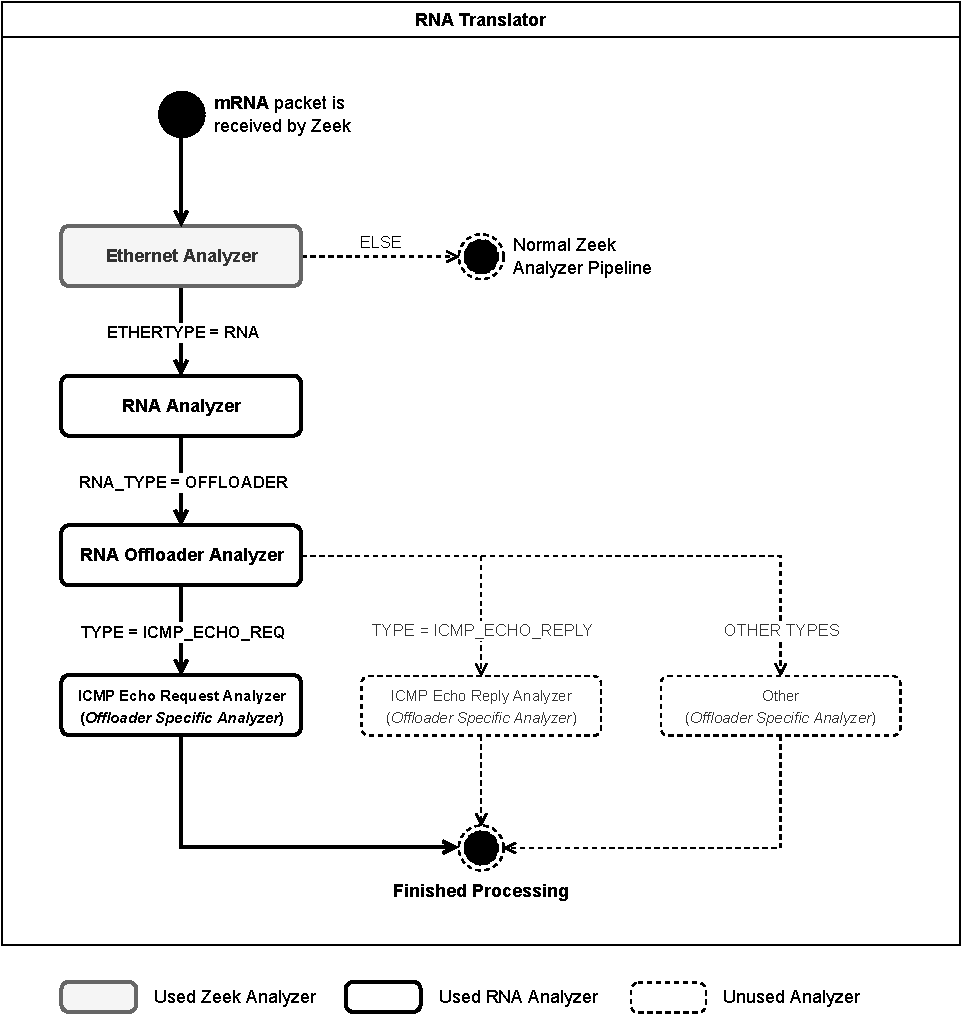
\includegraphics[width=0.8\textwidth]{images/icmp_ex_translator.pdf}  
    \end{center}
    \label{fig:icmp_ex_translator}
    \legend{Source: the author}
\end{figure}

The RNA Analyzer is the first Analyzer of the RNA architecture to receive the mRNA packet. As explained in the previous section, the RNA protocol has a generic header that indicates only the protocol version and the message type. This is the header that is extracted by the first Analyzer. In the case of this project, the only message type we use is the \Offloader{} type\footnotemark. Using our previously described example of the ICMP ping, the mRNA packet created for the ICMP ping will have its type as \textsc{\Offloader{}}, forwarding it to the RNA Offloader Analyzer.

\footnotetext{There are actually three types of \Offloaders{}, but for simplification purposes, in this description we present the Offloader type as being one unique type.}

Next, the RNA Offloader Analyzer is the second Analyzer of our RNA implementation to receive the mRNA packet. It parses the header generated by the General Offloader Splicer with \Offloader{} generic information. This Analyzer is also responsible for forwarding the mRNA packet and its payload to the \Offloader{} specific Analyzer by using the \Offloader{} \texttt{type} code. In our example, the next Analyzer to be executed is the \textsc{ICMP Echo Request} Analyzer. It is also important to note we display in Figure \ref{fig:icmp_ex_translator} two other Analyzers, displayed with dashed borders, that are present in the deployment but were not triggered due to the \Offloader{} type of this specific example packet: \textsc{ICMP Echo Request}.

The last Analyzer to be executed is the Offloader Analyzer. This is a module every \Offloader{} must have. It is responsible for converting the received information to Zeek's native structures. It can then trigger one or more desired events, which will be consumed by the monitoring scripts. In our example, the \textsc{ICMP Echo Request Analyzer} is going to trigger Zeek's native \texttt{icmp\_echo\_request} event. By triggering this event, we ensure all scripts that use it will perform exactly as Zeek had processed the ICMP ping request entirely in its own infrastructure.

As explained previously, an Analyzer directly triggering a Zeek Event is the ideal case, but not always possible. In the cases this is not possible, the Analyzer has the option to extract the mRNA headers and forward the rest of the payload to another Zeek-provided Analyzer. This other Analyzer, which is already part of Zeek's infrastructure, can then analyze the packet and trigger the proper events.
